\documentclass[1p]{elsarticle_modified}
%\bibliographystyle{elsarticle-num}

%\usepackage[colorlinks]{hyperref}
%\usepackage{abbrmath_seonhwa} %\Abb, \Ascr, \Acal ,\Abf, \Afrak
\usepackage{amsfonts}
\usepackage{amssymb}
\usepackage{amsmath}
\usepackage{amsthm}
\usepackage{scalefnt}
\usepackage{amsbsy}
\usepackage{kotex}
\usepackage{caption}
\usepackage{subfig}
\usepackage{color}
\usepackage{graphicx}
\usepackage{xcolor} %% white, black, red, green, blue, cyan, magenta, yellow
\usepackage{float}
\usepackage{setspace}
\usepackage{hyperref}

\usepackage{tikz}
\usetikzlibrary{arrows}

\usepackage{multirow}
\usepackage{array} % fixed length table
\usepackage{hhline}

%%%%%%%%%%%%%%%%%%%%%
\makeatletter
\renewcommand*\env@matrix[1][\arraystretch]{%
	\edef\arraystretch{#1}%
	\hskip -\arraycolsep
	\let\@ifnextchar\new@ifnextchar
	\array{*\c@MaxMatrixCols c}}
\makeatother %https://tex.stackexchange.com/questions/14071/how-can-i-increase-the-line-spacing-in-a-matrix
%%%%%%%%%%%%%%%

\usepackage[normalem]{ulem}

\newcommand{\msout}[1]{\ifmmode\text{\sout{\ensuremath{#1}}}\else\sout{#1}\fi}
%SOURCE: \msout is \stkout macro in https://tex.stackexchange.com/questions/20609/strikeout-in-math-mode

\newcommand{\cancel}[1]{
	\ifmmode
	{\color{red}\msout{#1}}
	\else
	{\color{red}\sout{#1}}
	\fi
}

\newcommand{\add}[1]{
	{\color{blue}\uwave{#1}}
}

\newcommand{\replace}[2]{
	\ifmmode
	{\color{red}\msout{#1}}{\color{blue}\uwave{#2}}
	\else
	{\color{red}\sout{#1}}{\color{blue}\uwave{#2}}
	\fi
}

\newcommand{\Sol}{\mathcal{S}} %segment
\newcommand{\D}{D} %diagram
\newcommand{\A}{\mathcal{A}} %arc


%%%%%%%%%%%%%%%%%%%%%%%%%%%%%5 test

\def\sl{\operatorname{\textup{SL}}(2,\Cbb)}
\def\psl{\operatorname{\textup{PSL}}(2,\Cbb)}
\def\quan{\mkern 1mu \triangleright \mkern 1mu}

\theoremstyle{definition}
\newtheorem{thm}{Theorem}[section]
\newtheorem{prop}[thm]{Proposition}
\newtheorem{lem}[thm]{Lemma}
\newtheorem{ques}[thm]{Question}
\newtheorem{cor}[thm]{Corollary}
\newtheorem{defn}[thm]{Definition}
\newtheorem{exam}[thm]{Example}
\newtheorem{rmk}[thm]{Remark}
\newtheorem{alg}[thm]{Algorithm}

\newcommand{\I}{\sqrt{-1}}
\begin{document}

%\begin{frontmatter}
%
%\title{Boundary parabolic representations of knots up to 8 crossings}
%
%%% Group authors per affiliation:
%\author{Yunhi Cho} 
%\address{Department of Mathematics, University of Seoul, Seoul, Korea}
%\ead{yhcho@uos.ac.kr}
%
%
%\author{Seonhwa Kim} %\fnref{s_kim}}
%\address{Center for Geometry and Physics, Institute for Basic Science, Pohang, 37673, Korea}
%\ead{ryeona17@ibs.re.kr}
%
%\author{Hyuk Kim}
%\address{Department of Mathematical Sciences, Seoul National University, Seoul 08826, Korea}
%\ead{hyukkim@snu.ac.kr}
%
%\author{Seokbeom Yoon}
%\address{Department of Mathematical Sciences, Seoul National University, Seoul, 08826,  Korea}
%\ead{sbyoon15@snu.ac.kr}
%
%\begin{abstract}
%We find all boundary parabolic representation of knots up to 8 crossings.
%
%\end{abstract}
%\begin{keyword}
%    \MSC[2010] 57M25 
%\end{keyword}
%
%\end{frontmatter}

%\linenumbers
%\tableofcontents
%
\newcommand\colored[1]{\textcolor{white}{\rule[-0.35ex]{0.8em}{1.4ex}}\kern-0.8em\color{red} #1}%
%\newcommand\colored[1]{\textcolor{white}{ #1}\kern-2.17ex	\textcolor{white}{ #1}\kern-1.81ex	\textcolor{white}{ #1}\kern-2.15ex\color{red}#1	}

{\Large $\underline{12n_{0223}~(K12n_{0223})}$}

\setlength{\tabcolsep}{10pt}
\renewcommand{\arraystretch}{1.6}
\vspace{1cm}\begin{tabular}{m{100pt}>{\centering\arraybackslash}m{274pt}}
\multirow{5}{120pt}{
	\centering
	\includegraphics[width=112pt]{../../../GIT/diagram.site/Diagrams/png/2312_12n_0223.png}\\
\ \ \ A knot diagram\footnotemark}&
\allowdisplaybreaks
\textbf{Linearized knot diagam} \\
\cline{2-2}
 &
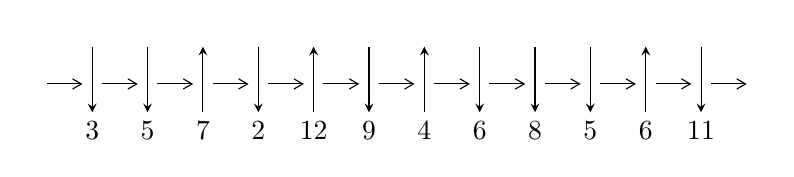
\begin{tikzpicture}[x=20pt, y=17pt]
	% nodes
	\node (C0) at (0, 0) {};
	\node (C1) at (1, 0) {};
	\node (C1U) at (1, +1) {};
	\node (C1D) at (1, -1) {3};

	\node (C2) at (2, 0) {};
	\node (C2U) at (2, +1) {};
	\node (C2D) at (2, -1) {5};

	\node (C3) at (3, 0) {};
	\node (C3U) at (3, +1) {};
	\node (C3D) at (3, -1) {7};

	\node (C4) at (4, 0) {};
	\node (C4U) at (4, +1) {};
	\node (C4D) at (4, -1) {2};

	\node (C5) at (5, 0) {};
	\node (C5U) at (5, +1) {};
	\node (C5D) at (5, -1) {12};

	\node (C6) at (6, 0) {};
	\node (C6U) at (6, +1) {};
	\node (C6D) at (6, -1) {9};

	\node (C7) at (7, 0) {};
	\node (C7U) at (7, +1) {};
	\node (C7D) at (7, -1) {4};

	\node (C8) at (8, 0) {};
	\node (C8U) at (8, +1) {};
	\node (C8D) at (8, -1) {6};

	\node (C9) at (9, 0) {};
	\node (C9U) at (9, +1) {};
	\node (C9D) at (9, -1) {8};

	\node (C10) at (10, 0) {};
	\node (C10U) at (10, +1) {};
	\node (C10D) at (10, -1) {5};

	\node (C11) at (11, 0) {};
	\node (C11U) at (11, +1) {};
	\node (C11D) at (11, -1) {6};

	\node (C12) at (12, 0) {};
	\node (C12U) at (12, +1) {};
	\node (C12D) at (12, -1) {11};
	\node (C13) at (13, 0) {};

	% arrows
	\draw[->,>={angle 60}]
	(C0) edge (C1) (C1) edge (C2) (C2) edge (C3) (C3) edge (C4) (C4) edge (C5) (C5) edge (C6) (C6) edge (C7) (C7) edge (C8) (C8) edge (C9) (C9) edge (C10) (C10) edge (C11) (C11) edge (C12) (C12) edge (C13) ;	\draw[->,>=stealth]
	(C1U) edge (C1D) (C2U) edge (C2D) (C3D) edge (C3U) (C4U) edge (C4D) (C5D) edge (C5U) (C6U) edge (C6D) (C7D) edge (C7U) (C8U) edge (C8D) (C9U) edge (C9D) (C10U) edge (C10D) (C11D) edge (C11U) (C12U) edge (C12D) ;
	\end{tikzpicture} \\
\hhline{~~} \\& 
\textbf{Solving Sequence} \\ \cline{2-2} 
 &
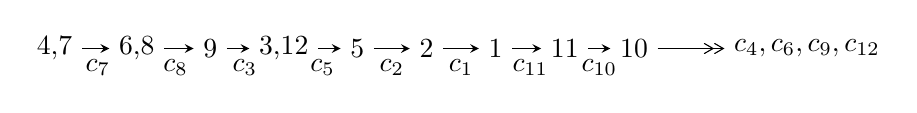
\begin{tikzpicture}[x=25pt, y=7pt]
	% node
	\node (A0) at (-1/8, 0) {4,7};
	\node (A1) at (17/16, 0) {6,8};
	\node (A2) at (17/8, 0) {9};
	\node (A3) at (51/16, 0) {3,12};
	\node (A4) at (17/4, 0) {5};
	\node (A5) at (21/4, 0) {2};
	\node (A6) at (25/4, 0) {1};
	\node (A7) at (29/4, 0) {11};
	\node (A8) at (33/4, 0) {10};
	\node (C1) at (1/2, -1) {$c_{7}$};
	\node (C2) at (13/8, -1) {$c_{8}$};
	\node (C3) at (21/8, -1) {$c_{3}$};
	\node (C4) at (15/4, -1) {$c_{5}$};
	\node (C5) at (19/4, -1) {$c_{2}$};
	\node (C6) at (23/4, -1) {$c_{1}$};
	\node (C7) at (27/4, -1) {$c_{11}$};
	\node (C8) at (31/4, -1) {$c_{10}$};
	\node (A9) at (43/4, 0) {$c_{4},c_{6},c_{9},c_{12}$};

	% edge
	\draw[->,>=stealth]	
	(A0) edge (A1) (A1) edge (A2) (A2) edge (A3) (A3) edge (A4) (A4) edge (A5) (A5) edge (A6) (A6) edge (A7) (A7) edge (A8) ;
	\draw[->>,>={angle 60}]	
	(A8) edge (A9);
\end{tikzpicture} \\ 

\end{tabular} \\

\footnotetext{
The image of knot diagram is generated by the software ``\textbf{Draw programme}" developed by Andrew Bartholomew(\url{http://www.layer8.co.uk/maths/draw/index.htm\#Running-draw}), where we modified some parts for our purpose(\url{https://github.com/CATsTAILs/LinksPainter}).
}\phantom \\ \newline 
\centering \textbf{Ideals for irreducible components\footnotemark of $X_{\text{par}}$} 
 
\begin{align*}
I^u_{1}&=\langle 
-1.05608\times10^{32} u^{27}+2.39983\times10^{32} u^{26}+\cdots+4.71199\times10^{33} d-1.14579\times10^{30},\\
\phantom{I^u_{1}}&\phantom{= \langle  }-7.16121\times10^{28} u^{27}+2.11432\times10^{32} u^{26}+\cdots+9.42397\times10^{33} c+9.50662\times10^{33},\\
\phantom{I^u_{1}}&\phantom{= \langle  }7.43837\times10^{31} u^{27}-2.05180\times10^{32} u^{26}+\cdots+4.71199\times10^{33} b-3.81499\times10^{32},\\
\phantom{I^u_{1}}&\phantom{= \langle  }5.68907\times10^{31} u^{27}-1.81131\times10^{32} u^{26}+\cdots+1.88479\times10^{34} a-1.63326\times10^{34},\;u^{28}-3 u^{27}+\cdots-64 u+32\rangle \\
I^u_{2}&=\langle 
-7778149750 u^{19} a+21085480149 u^{19}+\cdots+37111822100 a-70739740318,\\
\phantom{I^u_{2}}&\phantom{= \langle  }18555911050 u^{19} a-33847094283 u^{19}+\cdots-266919956828 a+210342367834,\\
\phantom{I^u_{2}}&\phantom{= \langle  }4182326921 u^{19} a+3076005459 u^{19}+\cdots-29433713862 a+28068851486,\\
\phantom{I^u_{2}}&\phantom{= \langle  }49133842327 u^{19} a-33157787379 u^{19}+\cdots-204672432210 a+75288972938,\\
\phantom{I^u_{2}}&\phantom{= \langle  }u^{20}+u^{19}+\cdots-8 u-4\rangle \\
\\
I^v_{1}&=\langle 
c,\;d- v,\;b,\;a-1,\;v^2+v+1\rangle \\
I^v_{2}&=\langle 
a,\;d+v,\;- a v+c- v-1,\;b+1,\;v^2+v+1\rangle \\
I^v_{3}&=\langle 
a,\;d-1,\;c+a,\;b+1,\;v+1\rangle \\
I^v_{4}&=\langle 
a,\;d^2 a+d^2 v+d c- d v- d+v+1,\;d^2 v^2- v^2 d- d v+v^2+2 v+1,\\
\phantom{I^v_{4}}&\phantom{= \langle  }d c a+d c v- d a- d v+c^2- c v- a v-2 c- a+1,\;v^2 d c- v^2 d- v^2 c- v^2 a- c v-2 a v- a,\\
\phantom{I^v_{4}}&\phantom{= \langle  }d a v+d a+d v+c v+c- v-1,\;c^2 v^2+v^2 c a+a^2 v^2+c a v- v^2 c+2 a^2 v+v^2 a+a^2+a v+v^2,\;b+1\rangle \\
\end{align*}
\raggedright * 5 irreducible components of $\dim_{\mathbb{C}}=0$, with total 73 representations.\\
\raggedright * 1 irreducible components of $\dim_{\mathbb{C}}=1$ \\
\footnotetext{All coefficients of polynomials are rational numbers. But the coefficients are sometimes approximated in decimal forms when there is not enough margin.}
\newpage
\renewcommand{\arraystretch}{1}
\centering \section*{I. $I^u_{1}= \langle -1.06\times10^{32} u^{27}+2.40\times10^{32} u^{26}+\cdots+4.71\times10^{33} d-1.15\times10^{30},\;-7.16\times10^{28} u^{27}+2.11\times10^{32} u^{26}+\cdots+9.42\times10^{33} c+9.51\times10^{33},\;7.44\times10^{31} u^{27}-2.05\times10^{32} u^{26}+\cdots+4.71\times10^{33} b-3.81\times10^{32},\;5.69\times10^{31} u^{27}-1.81\times10^{32} u^{26}+\cdots+1.88\times10^{34} a-1.63\times10^{34},\;u^{28}-3 u^{27}+\cdots-64 u+32 \rangle$}
\flushleft \textbf{(i) Arc colorings}\\
\begin{tabular}{m{7pt} m{180pt} m{7pt} m{180pt} }
\flushright $a_{4}=$&$\begin{pmatrix}0\\u\end{pmatrix}$ \\
\flushright $a_{7}=$&$\begin{pmatrix}1\\0\end{pmatrix}$ \\
\flushright $a_{6}=$&$\begin{pmatrix}-0.00301840 u^{27}+0.00961014 u^{26}+\cdots-0.512168 u+0.866547\\-0.0157861 u^{27}+0.0435442 u^{26}+\cdots-1.70037 u+0.0809635\end{pmatrix}$ \\
\flushright $a_{8}=$&$\begin{pmatrix}1\\- u^2\end{pmatrix}$ \\
\flushright $a_{9}=$&$\begin{pmatrix}-0.00301840 u^{27}+0.00961014 u^{26}+\cdots-0.512168 u+0.866547\\0.0152750 u^{27}-0.0402637 u^{26}+\cdots+1.56827 u-0.0632056\end{pmatrix}$ \\
\flushright $a_{3}=$&$\begin{pmatrix}- u\\u\end{pmatrix}$ \\
\flushright $a_{12}=$&$\begin{pmatrix}7.59893\times10^{-6} u^{27}-0.0224355 u^{26}+\cdots+3.09707 u-1.00877\\0.0224127 u^{27}-0.0509304 u^{26}+\cdots+1.00828 u+0.000243166\end{pmatrix}$ \\
\flushright $a_{5}=$&$\begin{pmatrix}-0.00253011 u^{27}-0.00819574 u^{26}+\cdots+1.54524 u-1.53844\\0.000554935 u^{27}-0.00115373 u^{26}+\cdots+0.673369 u+0.0965888\end{pmatrix}$ \\
\flushright $a_{2}=$&$\begin{pmatrix}0.00197517 u^{27}+0.00934947 u^{26}+\cdots-2.21861 u+1.44185\\0.000554935 u^{27}-0.00115373 u^{26}+\cdots+0.673369 u+0.0965888\end{pmatrix}$ \\
\flushright $a_{1}=$&$\begin{pmatrix}0.00578915 u^{27}-0.00833409 u^{26}+\cdots-1.28926 u+0.936700\\-0.00325904 u^{27}+0.0165298 u^{26}+\cdots-0.255976 u+0.601743\end{pmatrix}$ \\
\flushright $a_{11}=$&$\begin{pmatrix}-0.00186302 u^{27}-0.00814762 u^{26}+\cdots+1.14940 u-0.178203\\0.0260420 u^{27}-0.0682809 u^{26}+\cdots+2.68644 u-0.560928\end{pmatrix}$ \\
\flushright $a_{10}=$&$\begin{pmatrix}-0.0188045 u^{27}+0.0531544 u^{26}+\cdots-2.21254 u+0.947510\\0.00903337 u^{27}-0.0298398 u^{26}+\cdots+1.30721 u-0.185253\end{pmatrix}$\\&\end{tabular}
\flushleft \textbf{(ii) Obstruction class $= -1$}\\~\\
\flushleft \textbf{(iii) Cusp Shapes $= -0.217306 u^{27}+0.532528 u^{26}+\cdots-20.8205 u-2.69421$}\\~\\
\newpage\renewcommand{\arraystretch}{1}
\flushleft \textbf{(iv) u-Polynomials at the component}\newline \\
\begin{tabular}{m{50pt}|m{274pt}}
Crossings & \hspace{64pt}u-Polynomials at each crossing \\
\hline $$\begin{aligned}c_{1},c_{9}\end{aligned}$$&$\begin{aligned}
&u^{28}+9 u^{27}+\cdots+u+1
\end{aligned}$\\
\hline $$\begin{aligned}c_{2},c_{4},c_{6}\\c_{8}\end{aligned}$$&$\begin{aligned}
&u^{28}-5 u^{27}+\cdots-3 u+1
\end{aligned}$\\
\hline $$\begin{aligned}c_{3},c_{7}\end{aligned}$$&$\begin{aligned}
&u^{28}-3 u^{27}+\cdots-64 u+32
\end{aligned}$\\
\hline $$\begin{aligned}c_{5},c_{11}\end{aligned}$$&$\begin{aligned}
&u^{28}+u^{27}+\cdots+8 u+4
\end{aligned}$\\
\hline $$\begin{aligned}c_{10}\end{aligned}$$&$\begin{aligned}
&u^{28}- u^{27}+\cdots+1736 u+1252
\end{aligned}$\\
\hline $$\begin{aligned}c_{12}\end{aligned}$$&$\begin{aligned}
&u^{28}+9 u^{27}+\cdots-56 u+16
\end{aligned}$\\
\hline
\end{tabular}\\~\\
\newpage\renewcommand{\arraystretch}{1}
\flushleft \textbf{(v) Riley Polynomials at the component}\newline \\
\begin{tabular}{m{50pt}|m{274pt}}
Crossings & \hspace{64pt}Riley Polynomials at each crossing \\
\hline $$\begin{aligned}c_{1},c_{9}\end{aligned}$$&$\begin{aligned}
&y^{28}+31 y^{27}+\cdots+39 y+1
\end{aligned}$\\
\hline $$\begin{aligned}c_{2},c_{4},c_{6}\\c_{8}\end{aligned}$$&$\begin{aligned}
&y^{28}-9 y^{27}+\cdots- y+1
\end{aligned}$\\
\hline $$\begin{aligned}c_{3},c_{7}\end{aligned}$$&$\begin{aligned}
&y^{28}-15 y^{27}+\cdots+3072 y+1024
\end{aligned}$\\
\hline $$\begin{aligned}c_{5},c_{11}\end{aligned}$$&$\begin{aligned}
&y^{28}+9 y^{27}+\cdots-56 y+16
\end{aligned}$\\
\hline $$\begin{aligned}c_{10}\end{aligned}$$&$\begin{aligned}
&y^{28}+33 y^{27}+\cdots-17874936 y+1567504
\end{aligned}$\\
\hline $$\begin{aligned}c_{12}\end{aligned}$$&$\begin{aligned}
&y^{28}+21 y^{27}+\cdots-6432 y+256
\end{aligned}$\\
\hline
\end{tabular}\\~\\
\newpage\flushleft \textbf{(vi) Complex Volumes and Cusp Shapes}
$$\begin{array}{c|c|c}  
\text{Solutions to }I^u_{1}& \I (\text{vol} + \sqrt{-1}CS) & \text{Cusp shape}\\
 \hline 
\begin{aligned}
u &= \phantom{-}0.387721 + 0.851263 I \\
a &= \phantom{-}0.488405 - 0.103669 I \\
b &= -0.747142 - 0.797802 I \\
c &= -0.79488 - 1.41620 I \\
d &= -0.89737 + 1.22574 I\end{aligned}
 & -4.11180 - 3.97036 I & -11.03599 + 5.92521 I \\ \hline\begin{aligned}
u &= \phantom{-}0.387721 - 0.851263 I \\
a &= \phantom{-}0.488405 + 0.103669 I \\
b &= -0.747142 + 0.797802 I \\
c &= -0.79488 + 1.41620 I \\
d &= -0.89737 - 1.22574 I\end{aligned}
 & -4.11180 + 3.97036 I & -11.03599 - 5.92521 I \\ \hline\begin{aligned}
u &= -0.048850 + 0.802561 I \\
a &= \phantom{-}0.570907 + 0.125829 I \\
b &= -0.313957 + 0.493682 I \\
c &= \phantom{-}0.167451 + 0.444862 I \\
d &= \phantom{-}0.365209 - 0.112658 I\end{aligned}
 & -1.00554 + 1.45329 I & -3.70692 - 4.69342 I \\ \hline\begin{aligned}
u &= -0.048850 - 0.802561 I \\
a &= \phantom{-}0.570907 - 0.125829 I \\
b &= -0.313957 - 0.493682 I \\
c &= \phantom{-}0.167451 - 0.444862 I \\
d &= \phantom{-}0.365209 + 0.112658 I\end{aligned}
 & -1.00554 - 1.45329 I & -3.70692 + 4.69342 I \\ \hline\begin{aligned}
u &= \phantom{-}1.195800 + 0.230197 I \\
a &= \phantom{-}0.28063 - 1.44187 I \\
b &= -0.310268 + 1.162650 I \\
c &= \phantom{-}1.94455 - 0.47579 I \\
d &= -2.43482 + 0.12132 I\end{aligned}
 & \phantom{-}0.294538 + 1.243650 I & -3.92766 - 2.52803 I \\ \hline\begin{aligned}
u &= \phantom{-}1.195800 - 0.230197 I \\
a &= \phantom{-}0.28063 + 1.44187 I \\
b &= -0.310268 - 1.162650 I \\
c &= \phantom{-}1.94455 + 0.47579 I \\
d &= -2.43482 - 0.12132 I\end{aligned}
 & \phantom{-}0.294538 - 1.243650 I & -3.92766 + 2.52803 I\\
 \hline 
 \end{array}$$\newpage$$\begin{array}{c|c|c}  
\text{Solutions to }I^u_{1}& \I (\text{vol} + \sqrt{-1}CS) & \text{Cusp shape}\\
 \hline 
\begin{aligned}
u &= \phantom{-}0.512543 + 0.548760 I \\
a &= \phantom{-}0.810755 + 0.367303 I \\
b &= \phantom{-}0.214405 + 0.021676 I \\
c &= \phantom{-}1.012830 - 0.121876 I \\
d &= -0.586000 - 0.493336 I\end{aligned}
 & \phantom{-}0.77284 + 1.38296 I & \phantom{-}2.12358 - 4.20585 I \\ \hline\begin{aligned}
u &= \phantom{-}0.512543 - 0.548760 I \\
a &= \phantom{-}0.810755 - 0.367303 I \\
b &= \phantom{-}0.214405 - 0.021676 I \\
c &= \phantom{-}1.012830 + 0.121876 I \\
d &= -0.586000 + 0.493336 I\end{aligned}
 & \phantom{-}0.77284 - 1.38296 I & \phantom{-}2.12358 + 4.20585 I \\ \hline\begin{aligned}
u &= \phantom{-}1.240340 + 0.558685 I \\
a &= -0.19285 - 1.48947 I \\
b &= -0.74229 + 1.43353 I \\
c &= -2.20653 - 0.25596 I \\
d &= \phantom{-}2.59385 + 1.55023 I\end{aligned}
 & -1.36469 + 9.34331 I & -7.27750 - 7.90351 I \\ \hline\begin{aligned}
u &= \phantom{-}1.240340 - 0.558685 I \\
a &= -0.19285 + 1.48947 I \\
b &= -0.74229 - 1.43353 I \\
c &= -2.20653 + 0.25596 I \\
d &= \phantom{-}2.59385 - 1.55023 I\end{aligned}
 & -1.36469 - 9.34331 I & -7.27750 + 7.90351 I \\ \hline\begin{aligned}
u &= -0.306891 + 1.332240 I \\
a &= \phantom{-}0.448937 + 0.172706 I \\
b &= -0.32703 + 1.40380 I \\
c &= -0.489703 - 0.253197 I \\
d &= -0.487603 + 0.574696 I\end{aligned}
 & \phantom{-}2.80790 + 2.77377 I & -2.82329 - 2.35775 I \\ \hline\begin{aligned}
u &= -0.306891 - 1.332240 I \\
a &= \phantom{-}0.448937 - 0.172706 I \\
b &= -0.32703 - 1.40380 I \\
c &= -0.489703 + 0.253197 I \\
d &= -0.487603 - 0.574696 I\end{aligned}
 & \phantom{-}2.80790 - 2.77377 I & -2.82329 + 2.35775 I\\
 \hline 
 \end{array}$$\newpage$$\begin{array}{c|c|c}  
\text{Solutions to }I^u_{1}& \I (\text{vol} + \sqrt{-1}CS) & \text{Cusp shape}\\
 \hline 
\begin{aligned}
u &= -0.599185 + 0.160658 I \\
a &= \phantom{-}1.279080 - 0.454824 I \\
b &= -0.032693 + 0.151013 I \\
c &= \phantom{-}0.283924 - 1.075350 I \\
d &= -0.002639 - 0.689945 I\end{aligned}
 & -0.29820 + 2.58448 I & \phantom{-}1.60498 - 4.48843 I \\ \hline\begin{aligned}
u &= -0.599185 - 0.160658 I \\
a &= \phantom{-}1.279080 + 0.454824 I \\
b &= -0.032693 - 0.151013 I \\
c &= \phantom{-}0.283924 + 1.075350 I \\
d &= -0.002639 + 0.689945 I\end{aligned}
 & -0.29820 - 2.58448 I & \phantom{-}1.60498 + 4.48843 I \\ \hline\begin{aligned}
u &= \phantom{-}0.449039 + 1.329150 I \\
a &= \phantom{-}0.437109 - 0.156367 I \\
b &= -0.53079 - 1.49203 I \\
c &= \phantom{-}0.884456 + 0.900024 I \\
d &= \phantom{-}0.79911 - 1.57972 I\end{aligned}
 & \phantom{-}2.18074 - 8.77807 I & -4.21049 + 7.13120 I \\ \hline\begin{aligned}
u &= \phantom{-}0.449039 - 1.329150 I \\
a &= \phantom{-}0.437109 + 0.156367 I \\
b &= -0.53079 + 1.49203 I \\
c &= \phantom{-}0.884456 - 0.900024 I \\
d &= \phantom{-}0.79911 + 1.57972 I\end{aligned}
 & \phantom{-}2.18074 + 8.77807 I & -4.21049 - 7.13120 I \\ \hline\begin{aligned}
u &= -1.36520 + 0.37405 I \\
a &= \phantom{-}0.022772 + 1.320010 I \\
b &= -0.40047 - 1.49490 I \\
c &= -0.019011 + 0.257960 I \\
d &= \phantom{-}0.070537 + 0.359277 I\end{aligned}
 & \phantom{-}3.38586 - 5.92225 I & -1.05943 + 5.53498 I \\ \hline\begin{aligned}
u &= -1.36520 - 0.37405 I \\
a &= \phantom{-}0.022772 - 1.320010 I \\
b &= -0.40047 + 1.49490 I \\
c &= -0.019011 - 0.257960 I \\
d &= \phantom{-}0.070537 - 0.359277 I\end{aligned}
 & \phantom{-}3.38586 + 5.92225 I & -1.05943 - 5.53498 I\\
 \hline 
 \end{array}$$\newpage$$\begin{array}{c|c|c}  
\text{Solutions to }I^u_{1}& \I (\text{vol} + \sqrt{-1}CS) & \text{Cusp shape}\\
 \hline 
\begin{aligned}
u &= \phantom{-}0.128781 + 0.527754 I \\
a &= \phantom{-}0.536628 - 0.033094 I \\
b &= -0.720363 - 0.196098 I \\
c &= \phantom{-}0.53943 + 1.55105 I \\
d &= \phantom{-}0.749102 - 0.484434 I\end{aligned}
 & -2.91457 + 1.71407 I & -11.28016 - 2.34859 I \\ \hline\begin{aligned}
u &= \phantom{-}0.128781 - 0.527754 I \\
a &= \phantom{-}0.536628 + 0.033094 I \\
b &= -0.720363 + 0.196098 I \\
c &= \phantom{-}0.53943 - 1.55105 I \\
d &= \phantom{-}0.749102 + 0.484434 I\end{aligned}
 & -2.91457 - 1.71407 I & -11.28016 + 2.34859 I \\ \hline\begin{aligned}
u &= \phantom{-}1.36013 + 0.80195 I \\
a &= -0.423558 - 1.271240 I \\
b &= -1.02615 + 1.75013 I \\
c &= \phantom{-}1.77646 + 0.86372 I \\
d &= -1.72355 - 2.59940 I\end{aligned}
 & \phantom{-}5.1047 + 16.3284 I & -4.49305 - 9.50798 I \\ \hline\begin{aligned}
u &= \phantom{-}1.36013 - 0.80195 I \\
a &= -0.423558 + 1.271240 I \\
b &= -1.02615 - 1.75013 I \\
c &= \phantom{-}1.77646 - 0.86372 I \\
d &= -1.72355 + 2.59940 I\end{aligned}
 & \phantom{-}5.1047 - 16.3284 I & -4.49305 + 9.50798 I \\ \hline\begin{aligned}
u &= -1.41454 + 0.73498 I \\
a &= -0.342095 + 1.249650 I \\
b &= -0.89493 - 1.79229 I \\
c &= \phantom{-}0.231981 - 0.161062 I \\
d &= \phantom{-}0.209770 - 0.398331 I\end{aligned}
 & \phantom{-}6.34910 - 10.12380 I & -2.60535 + 5.05088 I \\ \hline\begin{aligned}
u &= -1.41454 - 0.73498 I \\
a &= -0.342095 - 1.249650 I \\
b &= -0.89493 + 1.79229 I \\
c &= \phantom{-}0.231981 + 0.161062 I \\
d &= \phantom{-}0.209770 + 0.398331 I\end{aligned}
 & \phantom{-}6.34910 + 10.12380 I & -2.60535 - 5.05088 I\\
 \hline 
 \end{array}$$\newpage$$\begin{array}{c|c|c}  
\text{Solutions to }I^u_{1}& \I (\text{vol} + \sqrt{-1}CS) & \text{Cusp shape}\\
 \hline 
\begin{aligned}
u &= \phantom{-}1.57578 + 0.34473 I \\
a &= \phantom{-}0.317772 + 0.829753 I \\
b &= \phantom{-}0.74767 - 1.25595 I \\
c &= -1.012250 - 0.840874 I \\
d &= \phantom{-}1.30521 + 1.67398 I\end{aligned}
 & \phantom{-}9.40632 + 3.24641 I & \phantom{-}0.187126 - 1.202849 I \\ \hline\begin{aligned}
u &= \phantom{-}1.57578 - 0.34473 I \\
a &= \phantom{-}0.317772 - 0.829753 I \\
b &= \phantom{-}0.74767 + 1.25595 I \\
c &= -1.012250 + 0.840874 I \\
d &= \phantom{-}1.30521 - 1.67398 I\end{aligned}
 & \phantom{-}9.40632 - 3.24641 I & \phantom{-}0.187126 + 1.202849 I \\ \hline\begin{aligned}
u &= -1.61547 + 0.19947 I \\
a &= \phantom{-}0.265518 - 0.890486 I \\
b &= \phantom{-}0.58401 + 1.42833 I \\
c &= -0.318722 + 0.271187 I \\
d &= -0.460792 + 0.501668 I\end{aligned}
 & \phantom{-}9.82407 + 3.16258 I & \phantom{-}0.50415 - 3.81889 I \\ \hline\begin{aligned}
u &= -1.61547 - 0.19947 I \\
a &= \phantom{-}0.265518 + 0.890486 I \\
b &= \phantom{-}0.58401 - 1.42833 I \\
c &= -0.318722 - 0.271187 I \\
d &= -0.460792 - 0.501668 I\end{aligned}
 & \phantom{-}9.82407 - 3.16258 I & \phantom{-}0.50415 + 3.81889 I\\
 \hline 
 \end{array}$$\newpage\newpage\renewcommand{\arraystretch}{1}
\centering \section*{II. $I^u_{2}= \langle -7.78\times10^{9} a u^{19}+2.11\times10^{10} u^{19}+\cdots+3.71\times10^{10} a-7.07\times10^{10},\;1.86\times10^{10} a u^{19}-3.38\times10^{10} u^{19}+\cdots-2.67\times10^{11} a+2.10\times10^{11},\;4.18\times10^{9} a u^{19}+3.08\times10^{9} u^{19}+\cdots-2.94\times10^{10} a+2.81\times10^{10},\;4.91\times10^{10} a u^{19}-3.32\times10^{10} u^{19}+\cdots-2.05\times10^{11} a+7.53\times10^{10},\;u^{20}+u^{19}+\cdots-8 u-4 \rangle$}
\flushleft \textbf{(i) Arc colorings}\\
\begin{tabular}{m{7pt} m{180pt} m{7pt} m{180pt} }
\flushright $a_{4}=$&$\begin{pmatrix}0\\u\end{pmatrix}$ \\
\flushright $a_{7}=$&$\begin{pmatrix}1\\0\end{pmatrix}$ \\
\flushright $a_{6}=$&$\begin{pmatrix}a\\-0.154609 a u^{19}-0.113711 u^{19}+\cdots+1.08808 a-1.03762\end{pmatrix}$ \\
\flushright $a_{8}=$&$\begin{pmatrix}1\\- u^2\end{pmatrix}$ \\
\flushright $a_{9}=$&$\begin{pmatrix}a\\0.154609 a u^{19}+0.113711 u^{19}+\cdots-1.08808 a+1.03762\end{pmatrix}$ \\
\flushright $a_{3}=$&$\begin{pmatrix}- u\\u\end{pmatrix}$ \\
\flushright $a_{12}=$&$\begin{pmatrix}-0.171490 a u^{19}+0.312807 u^{19}+\cdots+2.46682 a-1.94394\\0.143768 a u^{19}-0.389735 u^{19}+\cdots-0.685959 a+1.30752\end{pmatrix}$ \\
\flushright $a_{5}=$&$\begin{pmatrix}-0.272020 a u^{19}+0.0220200 u^{19}+\cdots+2.18366 a-0.183663\\0.227980 u^{19}+0.382589 u^{18}+\cdots-1.74114 u-1.81634\end{pmatrix}$ \\
\flushright $a_{2}=$&$\begin{pmatrix}0.272020 a u^{19}-0.250000 u^{19}+\cdots-2.18366 a+2\\0.227980 u^{19}+0.382589 u^{18}+\cdots-1.74114 u-1.81634\end{pmatrix}$ \\
\flushright $a_{1}=$&$\begin{pmatrix}0.392720 a u^{19}-0.370700 u^{19}+\cdots-2.80210 a+2.61843\\-0.120700 a u^{19}+0.348680 u^{19}+\cdots+0.618434 a-2.43477\end{pmatrix}$ \\
\flushright $a_{11}=$&$\begin{pmatrix}-0.486024 a u^{19}+0.312807 u^{19}+\cdots+3.53102 a-1.94394\\0.345654 a u^{19}-0.0895665 u^{19}+\cdots-1.54407 a+0.431179\end{pmatrix}$ \\
\flushright $a_{10}=$&$\begin{pmatrix}-0.154609 a u^{19}-0.113711 u^{19}+\cdots+2.08808 a-1.03762\\0.409919 a u^{19}+0.367791 u^{19}+\cdots-1.57088 a+0.0883006\end{pmatrix}$\\&\end{tabular}
\flushleft \textbf{(ii) Obstruction class $= -1$}\\~\\
\flushleft \textbf{(iii) Cusp Shapes $= -\frac{4263121051}{13525530286} u^{19}-\frac{7308875275}{13525530286} u^{18}+\cdots+\frac{12379392387}{13525530286} u-\frac{17100277556}{6762765143}$}\\~\\
\newpage\renewcommand{\arraystretch}{1}
\flushleft \textbf{(iv) u-Polynomials at the component}\newline \\
\begin{tabular}{m{50pt}|m{274pt}}
Crossings & \hspace{64pt}u-Polynomials at each crossing \\
\hline $$\begin{aligned}c_{1},c_{9}\end{aligned}$$&$\begin{aligned}
&u^{40}+19 u^{39}+\cdots+288 u+256
\end{aligned}$\\
\hline $$\begin{aligned}c_{2},c_{4},c_{6}\\c_{8}\end{aligned}$$&$\begin{aligned}
&u^{40}-3 u^{39}+\cdots+40 u-16
\end{aligned}$\\
\hline $$\begin{aligned}c_{3},c_{7}\end{aligned}$$&$\begin{aligned}
&(u^{20}+u^{19}+\cdots-8 u-4)^{2}
\end{aligned}$\\
\hline $$\begin{aligned}c_{5},c_{11}\end{aligned}$$&$\begin{aligned}
&(u^{20}+2 u^{19}+\cdots-2 u+1)^{2}
\end{aligned}$\\
\hline $$\begin{aligned}c_{10}\end{aligned}$$&$\begin{aligned}
&(u^{20}-2 u^{19}+\cdots+36 u+17)^{2}
\end{aligned}$\\
\hline $$\begin{aligned}c_{12}\end{aligned}$$&$\begin{aligned}
&(u^{20}+6 u^{19}+\cdots-2 u+1)^{2}
\end{aligned}$\\
\hline
\end{tabular}\\~\\
\newpage\renewcommand{\arraystretch}{1}
\flushleft \textbf{(v) Riley Polynomials at the component}\newline \\
\begin{tabular}{m{50pt}|m{274pt}}
Crossings & \hspace{64pt}Riley Polynomials at each crossing \\
\hline $$\begin{aligned}c_{1},c_{9}\end{aligned}$$&$\begin{aligned}
&y^{40}+y^{39}+\cdots-4022784 y+65536
\end{aligned}$\\
\hline $$\begin{aligned}c_{2},c_{4},c_{6}\\c_{8}\end{aligned}$$&$\begin{aligned}
&y^{40}-19 y^{39}+\cdots-288 y+256
\end{aligned}$\\
\hline $$\begin{aligned}c_{3},c_{7}\end{aligned}$$&$\begin{aligned}
&(y^{20}-15 y^{19}+\cdots-24 y+16)^{2}
\end{aligned}$\\
\hline $$\begin{aligned}c_{5},c_{11}\end{aligned}$$&$\begin{aligned}
&(y^{20}+6 y^{19}+\cdots-2 y+1)^{2}
\end{aligned}$\\
\hline $$\begin{aligned}c_{10}\end{aligned}$$&$\begin{aligned}
&(y^{20}+30 y^{19}+\cdots+1254 y+289)^{2}
\end{aligned}$\\
\hline $$\begin{aligned}c_{12}\end{aligned}$$&$\begin{aligned}
&(y^{20}+18 y^{19}+\cdots-86 y+1)^{2}
\end{aligned}$\\
\hline
\end{tabular}\\~\\
\newpage\flushleft \textbf{(vi) Complex Volumes and Cusp Shapes}
$$\begin{array}{c|c|c}  
\text{Solutions to }I^u_{2}& \I (\text{vol} + \sqrt{-1}CS) & \text{Cusp shape}\\
 \hline 
\begin{aligned}
u &= \phantom{-}0.685016 + 0.443026 I \\
a &= \phantom{-}0.458140 - 0.042470 I \\
b &= -1.314980 - 0.467098 I \\
c &= -1.19123 - 1.35374 I \\
d &= \phantom{-}1.34492 + 3.28525 I\end{aligned}
 & -4.73160 + 1.82256 I & -11.12541 - 5.12436 I \\ \hline\begin{aligned}
u &= \phantom{-}0.685016 + 0.443026 I \\
a &= -0.09245 - 3.22238 I \\
b &= -0.921725 + 0.625666 I \\
c &= -3.57126 - 2.48620 I \\
d &= \phantom{-}0.21627 + 1.45508 I\end{aligned}
 & -4.73160 + 1.82256 I & -11.12541 - 5.12436 I \\ \hline\begin{aligned}
u &= \phantom{-}0.685016 - 0.443026 I \\
a &= \phantom{-}0.458140 + 0.042470 I \\
b &= -1.314980 + 0.467098 I \\
c &= -1.19123 + 1.35374 I \\
d &= \phantom{-}1.34492 - 3.28525 I\end{aligned}
 & -4.73160 - 1.82256 I & -11.12541 + 5.12436 I \\ \hline\begin{aligned}
u &= \phantom{-}0.685016 - 0.443026 I \\
a &= -0.09245 + 3.22238 I \\
b &= -0.921725 - 0.625666 I \\
c &= -3.57126 + 2.48620 I \\
d &= \phantom{-}0.21627 - 1.45508 I\end{aligned}
 & -4.73160 - 1.82256 I & -11.12541 + 5.12436 I \\ \hline\begin{aligned}
u &= -1.176520 + 0.244065 I \\
a &= \phantom{-}0.577483 - 0.947538 I \\
b &= \phantom{-}0.310218 + 0.817249 I \\
c &= \phantom{-}1.70100 - 0.02090 I \\
d &= -1.82568 + 1.36744 I\end{aligned}
 & \phantom{-}0.28251 - 3.88098 I & -3.93502 + 4.02252 I \\ \hline\begin{aligned}
u &= -1.176520 + 0.244065 I \\
a &= \phantom{-}0.27911 + 1.47852 I \\
b &= -0.342116 - 1.145120 I \\
c &= -1.71890 + 0.80569 I \\
d &= \phantom{-}1.99616 - 0.43974 I\end{aligned}
 & \phantom{-}0.28251 - 3.88098 I & -3.93502 + 4.02252 I\\
 \hline 
 \end{array}$$\newpage$$\begin{array}{c|c|c}  
\text{Solutions to }I^u_{2}& \I (\text{vol} + \sqrt{-1}CS) & \text{Cusp shape}\\
 \hline 
\begin{aligned}
u &= -1.176520 - 0.244065 I \\
a &= \phantom{-}0.577483 + 0.947538 I \\
b &= \phantom{-}0.310218 - 0.817249 I \\
c &= \phantom{-}1.70100 + 0.02090 I \\
d &= -1.82568 - 1.36744 I\end{aligned}
 & \phantom{-}0.28251 + 3.88098 I & -3.93502 - 4.02252 I \\ \hline\begin{aligned}
u &= -1.176520 - 0.244065 I \\
a &= \phantom{-}0.27911 - 1.47852 I \\
b &= -0.342116 + 1.145120 I \\
c &= -1.71890 - 0.80569 I \\
d &= \phantom{-}1.99616 + 0.43974 I\end{aligned}
 & \phantom{-}0.28251 + 3.88098 I & -3.93502 - 4.02252 I \\ \hline\begin{aligned}
u &= -1.256010 + 0.124886 I \\
a &= \phantom{-}0.339080 + 1.286040 I \\
b &= -0.124777 - 1.175340 I \\
c &= \phantom{-}0.00787 - 1.59574 I \\
d &= \phantom{-}0.528809 + 0.982333 I\end{aligned}
 & \phantom{-}1.249910 + 0.191668 I & -2.26430 + 0.22109 I \\ \hline\begin{aligned}
u &= -1.256010 + 0.124886 I \\
a &= \phantom{-}0.408592 + 0.009946 I \\
b &= -2.08731 + 0.17219 I \\
c &= \phantom{-}0.339897 + 0.815901 I \\
d &= -0.18941 - 2.00525 I\end{aligned}
 & \phantom{-}1.249910 + 0.191668 I & -2.26430 + 0.22109 I \\ \hline\begin{aligned}
u &= -1.256010 - 0.124886 I \\
a &= \phantom{-}0.339080 - 1.286040 I \\
b &= -0.124777 + 1.175340 I \\
c &= \phantom{-}0.00787 + 1.59574 I \\
d &= \phantom{-}0.528809 - 0.982333 I\end{aligned}
 & \phantom{-}1.249910 - 0.191668 I & -2.26430 - 0.22109 I \\ \hline\begin{aligned}
u &= -1.256010 - 0.124886 I \\
a &= \phantom{-}0.408592 - 0.009946 I \\
b &= -2.08731 - 0.17219 I \\
c &= \phantom{-}0.339897 - 0.815901 I \\
d &= -0.18941 + 2.00525 I\end{aligned}
 & \phantom{-}1.249910 - 0.191668 I & -2.26430 - 0.22109 I\\
 \hline 
 \end{array}$$\newpage$$\begin{array}{c|c|c}  
\text{Solutions to }I^u_{2}& \I (\text{vol} + \sqrt{-1}CS) & \text{Cusp shape}\\
 \hline 
\begin{aligned}
u &= \phantom{-}1.268400 + 0.295253 I \\
a &= \phantom{-}0.150939 - 1.397650 I \\
b &= -0.352887 + 1.306450 I \\
c &= \phantom{-}0.00100 + 1.90027 I \\
d &= -0.322075 - 1.194470 I\end{aligned}
 & \phantom{-}0.89345 + 5.67427 I & -3.40403 - 5.66395 I \\ \hline\begin{aligned}
u &= \phantom{-}1.268400 + 0.295253 I \\
a &= \phantom{-}0.406505 - 0.023413 I \\
b &= -2.08796 - 0.41006 I \\
c &= \phantom{-}0.448812 + 0.837239 I \\
d &= \phantom{-}0.55980 - 2.41060 I\end{aligned}
 & \phantom{-}0.89345 + 5.67427 I & -3.40403 - 5.66395 I \\ \hline\begin{aligned}
u &= \phantom{-}1.268400 - 0.295253 I \\
a &= \phantom{-}0.150939 + 1.397650 I \\
b &= -0.352887 - 1.306450 I \\
c &= \phantom{-}0.00100 - 1.90027 I \\
d &= -0.322075 + 1.194470 I\end{aligned}
 & \phantom{-}0.89345 - 5.67427 I & -3.40403 + 5.66395 I \\ \hline\begin{aligned}
u &= \phantom{-}1.268400 - 0.295253 I \\
a &= \phantom{-}0.406505 + 0.023413 I \\
b &= -2.08796 + 0.41006 I \\
c &= \phantom{-}0.448812 - 0.837239 I \\
d &= \phantom{-}0.55980 + 2.41060 I\end{aligned}
 & \phantom{-}0.89345 - 5.67427 I & -3.40403 + 5.66395 I \\ \hline\begin{aligned}
u &= -0.439566 + 0.534727 I \\
a &= \phantom{-}0.820860 - 0.314763 I \\
b &= \phantom{-}0.162005 - 0.050556 I \\
c &= \phantom{-}1.70038 - 0.48109 I \\
d &= \phantom{-}0.255350 + 0.690923 I\end{aligned}
 & -2.07115 + 0.86143 I & -6.44675 + 0.99952 I \\ \hline\begin{aligned}
u &= -0.439566 + 0.534727 I \\
a &= \phantom{-}0.487252 + 0.053221 I \\
b &= -1.007970 + 0.455517 I \\
c &= -0.536806 + 0.918810 I \\
d &= \phantom{-}0.490181 - 1.120710 I\end{aligned}
 & -2.07115 + 0.86143 I & -6.44675 + 0.99952 I\\
 \hline 
 \end{array}$$\newpage$$\begin{array}{c|c|c}  
\text{Solutions to }I^u_{2}& \I (\text{vol} + \sqrt{-1}CS) & \text{Cusp shape}\\
 \hline 
\begin{aligned}
u &= -0.439566 - 0.534727 I \\
a &= \phantom{-}0.820860 + 0.314763 I \\
b &= \phantom{-}0.162005 + 0.050556 I \\
c &= \phantom{-}1.70038 + 0.48109 I \\
d &= \phantom{-}0.255350 - 0.690923 I\end{aligned}
 & -2.07115 - 0.86143 I & -6.44675 - 0.99952 I \\ \hline\begin{aligned}
u &= -0.439566 - 0.534727 I \\
a &= \phantom{-}0.487252 - 0.053221 I \\
b &= -1.007970 - 0.455517 I \\
c &= -0.536806 - 0.918810 I \\
d &= \phantom{-}0.490181 + 1.120710 I\end{aligned}
 & -2.07115 - 0.86143 I & -6.44675 - 0.99952 I \\ \hline\begin{aligned}
u &= -0.089922 + 1.317200 I \\
a &= \phantom{-}0.481544 - 0.234697 I \\
b &= \phantom{-}0.209138 - 1.109080 I \\
c &= -0.377586 + 0.174434 I \\
d &= -0.78245 - 1.28050 I\end{aligned}
 & \phantom{-}3.24441 + 2.97363 I & -2.07664 - 2.68538 I \\ \hline\begin{aligned}
u &= -0.089922 + 1.317200 I \\
a &= \phantom{-}0.469189 + 0.202331 I \\
b &= -0.034817 + 1.235550 I \\
c &= \phantom{-}0.927267 - 0.657327 I \\
d &= \phantom{-}0.195810 + 0.513040 I\end{aligned}
 & \phantom{-}3.24441 + 2.97363 I & -2.07664 - 2.68538 I \\ \hline\begin{aligned}
u &= -0.089922 - 1.317200 I \\
a &= \phantom{-}0.481544 + 0.234697 I \\
b &= \phantom{-}0.209138 + 1.109080 I \\
c &= -0.377586 - 0.174434 I \\
d &= -0.78245 + 1.28050 I\end{aligned}
 & \phantom{-}3.24441 - 2.97363 I & -2.07664 + 2.68538 I \\ \hline\begin{aligned}
u &= -0.089922 - 1.317200 I \\
a &= \phantom{-}0.469189 - 0.202331 I \\
b &= -0.034817 - 1.235550 I \\
c &= \phantom{-}0.927267 + 0.657327 I \\
d &= \phantom{-}0.195810 - 0.513040 I\end{aligned}
 & \phantom{-}3.24441 - 2.97363 I & -2.07664 + 2.68538 I\\
 \hline 
 \end{array}$$\newpage$$\begin{array}{c|c|c}  
\text{Solutions to }I^u_{2}& \I (\text{vol} + \sqrt{-1}CS) & \text{Cusp shape}\\
 \hline 
\begin{aligned}
u &= \phantom{-}1.36144\phantom{ +0.000000I} \\
a &= \phantom{-}0.339214 + 1.109820 I \\
b &= \phantom{-}0.119387 - 1.233010 I \\
c &= \phantom{-}0.299266 + 0.242908 I \\
d &= -0.407433 + 0.330704 I\end{aligned}
 & \phantom{-}4.11381\phantom{ +0.000000I} & \phantom{-}0.668270\phantom{ +0.000000I} \\ \hline\begin{aligned}
u &= \phantom{-}1.36144\phantom{ +0.000000I} \\
a &= \phantom{-}0.339214 - 1.109820 I \\
b &= \phantom{-}0.119387 + 1.233010 I \\
c &= \phantom{-}0.299266 - 0.242908 I \\
d &= -0.407433 - 0.330704 I\end{aligned}
 & \phantom{-}4.11381\phantom{ +0.000000I} & \phantom{-}0.668270\phantom{ +0.000000I} \\ \hline\begin{aligned}
u &= -0.610309\phantom{ +0.000000I} \\
a &= \phantom{-}0.465000\phantom{ +0.000000I} \\
b &= -1.32374\phantom{ +0.000000I} \\
c &= -0.750025\phantom{ +0.000000I} \\
d &= \phantom{-}1.42139\phantom{ +0.000000I}\end{aligned}
 & -2.43031\phantom{ +0.000000I} & -0.135410\phantom{ +0.000000I} \\ \hline\begin{aligned}
u &= -0.610309\phantom{ +0.000000I} \\
a &= \phantom{-}2.94194\phantom{ +0.000000I} \\
b &= -0.435716\phantom{ +0.000000I} \\
c &= \phantom{-}2.32897\phantom{ +0.000000I} \\
d &= -0.457747\phantom{ +0.000000I}\end{aligned}
 & -2.43031\phantom{ +0.000000I} & -0.135410\phantom{ +0.000000I} \\ \hline\begin{aligned}
u &= \phantom{-}0.078647 + 0.574169 I \\
a &= \phantom{-}0.556867 - 0.032704 I \\
b &= -0.612405 - 0.165972 I \\
c &= \phantom{-}2.18886 - 0.63265 I \\
d &= -3.72549 + 1.36694 I\end{aligned}
 & -2.82359 - 2.30782 I & -10.11267 + 3.58910 I \\ \hline\begin{aligned}
u &= \phantom{-}0.078647 + 0.574169 I \\
a &= -7.02820 - 1.64334 I \\
b &= -1.287020 + 0.071600 I \\
c &= -1.46449 - 6.68908 I \\
d &= -0.535397 - 1.207020 I\end{aligned}
 & -2.82359 - 2.30782 I & -10.11267 + 3.58910 I\\
 \hline 
 \end{array}$$\newpage$$\begin{array}{c|c|c}  
\text{Solutions to }I^u_{2}& \I (\text{vol} + \sqrt{-1}CS) & \text{Cusp shape}\\
 \hline 
\begin{aligned}
u &= \phantom{-}0.078647 - 0.574169 I \\
a &= \phantom{-}0.556867 + 0.032704 I \\
b &= -0.612405 + 0.165972 I \\
c &= \phantom{-}2.18886 + 0.63265 I \\
d &= -3.72549 - 1.36694 I\end{aligned}
 & -2.82359 + 2.30782 I & -10.11267 - 3.58910 I \\ \hline\begin{aligned}
u &= \phantom{-}0.078647 - 0.574169 I \\
a &= -7.02820 + 1.64334 I \\
b &= -1.287020 - 0.071600 I \\
c &= -1.46449 + 6.68908 I \\
d &= -0.535397 + 1.207020 I\end{aligned}
 & -2.82359 + 2.30782 I & -10.11267 - 3.58910 I \\ \hline\begin{aligned}
u &= -1.47182 + 0.62184 I \\
a &= \phantom{-}0.387142 - 0.708904 I \\
b &= \phantom{-}1.015300 + 0.883621 I \\
c &= -1.36735 + 0.63910 I \\
d &= \phantom{-}1.04280 - 2.20163 I\end{aligned}
 & \phantom{-}7.69158 - 9.88458 I & -1.61748 + 5.77638 I \\ \hline\begin{aligned}
u &= -1.47182 + 0.62184 I \\
a &= -0.227488 + 1.225540 I \\
b &= -0.69209 - 1.80855 I \\
c &= \phantom{-}1.13747 - 1.01527 I \\
d &= -1.61508 + 1.79092 I\end{aligned}
 & \phantom{-}7.69158 - 9.88458 I & -1.61748 + 5.77638 I \\ \hline\begin{aligned}
u &= -1.47182 - 0.62184 I \\
a &= \phantom{-}0.387142 + 0.708904 I \\
b &= \phantom{-}1.015300 - 0.883621 I \\
c &= -1.36735 - 0.63910 I \\
d &= \phantom{-}1.04280 + 2.20163 I\end{aligned}
 & \phantom{-}7.69158 + 9.88458 I & -1.61748 - 5.77638 I \\ \hline\begin{aligned}
u &= -1.47182 - 0.62184 I \\
a &= -0.227488 - 1.225540 I \\
b &= -0.69209 + 1.80855 I \\
c &= \phantom{-}1.13747 + 1.01527 I \\
d &= -1.61508 - 1.79092 I\end{aligned}
 & \phantom{-}7.69158 + 9.88458 I & -1.61748 - 5.77638 I\\
 \hline 
 \end{array}$$\newpage$$\begin{array}{c|c|c}  
\text{Solutions to }I^u_{2}& \I (\text{vol} + \sqrt{-1}CS) & \text{Cusp shape}\\
 \hline 
\begin{aligned}
u &= \phantom{-}1.52621 + 0.50989 I \\
a &= \phantom{-}0.360132 + 0.757386 I \\
b &= \phantom{-}0.921521 - 1.050930 I \\
c &= -0.411289 + 0.112437 I \\
d &= \phantom{-}0.106033 - 0.813106 I\end{aligned}
 & \phantom{-}8.58220 + 3.56941 I & -0.284129 - 1.007355 I \\ \hline\begin{aligned}
u &= \phantom{-}1.52621 + 0.50989 I \\
a &= -0.127382 - 1.185430 I \\
b &= -0.49179 + 1.81736 I \\
c &= \phantom{-}0.097619 + 0.500148 I \\
d &= \phantom{-}0.685044 + 0.038109 I\end{aligned}
 & \phantom{-}8.58220 + 3.56941 I & -0.284129 - 1.007355 I \\ \hline\begin{aligned}
u &= \phantom{-}1.52621 - 0.50989 I \\
a &= \phantom{-}0.360132 - 0.757386 I \\
b &= \phantom{-}0.921521 + 1.050930 I \\
c &= -0.411289 - 0.112437 I \\
d &= \phantom{-}0.106033 + 0.813106 I\end{aligned}
 & \phantom{-}8.58220 - 3.56941 I & -0.284129 + 1.007355 I \\ \hline\begin{aligned}
u &= \phantom{-}1.52621 - 0.50989 I \\
a &= -0.127382 + 1.185430 I \\
b &= -0.49179 - 1.81736 I \\
c &= \phantom{-}0.097619 - 0.500148 I \\
d &= \phantom{-}0.685044 - 0.038109 I\end{aligned}
 & \phantom{-}8.58220 - 3.56941 I & -0.284129 + 1.007355 I\\
 \hline 
 \end{array}$$\newpage\newpage\renewcommand{\arraystretch}{1}
\centering \section*{III. $I^v_{1}= \langle c,\;d- v,\;b,\;a-1,\;v^2+v+1 \rangle$}
\flushleft \textbf{(i) Arc colorings}\\
\begin{tabular}{m{7pt} m{180pt} m{7pt} m{180pt} }
\flushright $a_{4}=$&$\begin{pmatrix}v\\0\end{pmatrix}$ \\
\flushright $a_{7}=$&$\begin{pmatrix}1\\0\end{pmatrix}$ \\
\flushright $a_{6}=$&$\begin{pmatrix}1\\0\end{pmatrix}$ \\
\flushright $a_{8}=$&$\begin{pmatrix}1\\0\end{pmatrix}$ \\
\flushright $a_{9}=$&$\begin{pmatrix}1\\0\end{pmatrix}$ \\
\flushright $a_{3}=$&$\begin{pmatrix}v\\0\end{pmatrix}$ \\
\flushright $a_{12}=$&$\begin{pmatrix}0\\v\end{pmatrix}$ \\
\flushright $a_{5}=$&$\begin{pmatrix}1\\- v-1\end{pmatrix}$ \\
\flushright $a_{2}=$&$\begin{pmatrix}v-1\\v+1\end{pmatrix}$ \\
\flushright $a_{1}=$&$\begin{pmatrix}-1\\v+1\end{pmatrix}$ \\
\flushright $a_{11}=$&$\begin{pmatrix}- v\\v\end{pmatrix}$ \\
\flushright $a_{10}=$&$\begin{pmatrix}1\\0\end{pmatrix}$\\&\end{tabular}
\flushleft \textbf{(ii) Obstruction class $= 1$}\\~\\
\flushleft \textbf{(iii) Cusp Shapes $= 4 v-1$}\\~\\
\newpage\renewcommand{\arraystretch}{1}
\flushleft \textbf{(iv) u-Polynomials at the component}\newline \\
\begin{tabular}{m{50pt}|m{274pt}}
Crossings & \hspace{64pt}u-Polynomials at each crossing \\
\hline $$\begin{aligned}c_{1},c_{2}\end{aligned}$$&$\begin{aligned}
&(u-1)^2
\end{aligned}$\\
\hline $$\begin{aligned}c_{3},c_{6},c_{7}\\c_{8},c_{9}\end{aligned}$$&$\begin{aligned}
&u^2
\end{aligned}$\\
\hline $$\begin{aligned}c_{4}\end{aligned}$$&$\begin{aligned}
&(u+1)^2
\end{aligned}$\\
\hline $$\begin{aligned}c_{5},c_{10},c_{12}\end{aligned}$$&$\begin{aligned}
&u^2+u+1
\end{aligned}$\\
\hline $$\begin{aligned}c_{11}\end{aligned}$$&$\begin{aligned}
&u^2- u+1
\end{aligned}$\\
\hline
\end{tabular}\\~\\
\newpage\renewcommand{\arraystretch}{1}
\flushleft \textbf{(v) Riley Polynomials at the component}\newline \\
\begin{tabular}{m{50pt}|m{274pt}}
Crossings & \hspace{64pt}Riley Polynomials at each crossing \\
\hline $$\begin{aligned}c_{1},c_{2},c_{4}\end{aligned}$$&$\begin{aligned}
&(y-1)^2
\end{aligned}$\\
\hline $$\begin{aligned}c_{3},c_{6},c_{7}\\c_{8},c_{9}\end{aligned}$$&$\begin{aligned}
&y^2
\end{aligned}$\\
\hline $$\begin{aligned}c_{5},c_{10},c_{11}\\c_{12}\end{aligned}$$&$\begin{aligned}
&y^2+y+1
\end{aligned}$\\
\hline
\end{tabular}\\~\\
\newpage\flushleft \textbf{(vi) Complex Volumes and Cusp Shapes}
$$\begin{array}{c|c|c}  
\text{Solutions to }I^v_{1}& \I (\text{vol} + \sqrt{-1}CS) & \text{Cusp shape}\\
 \hline 
\begin{aligned}
v &= -0.500000 + 0.866025 I \\
a &= \phantom{-}1.00000\phantom{ +0.000000I} \\
b &= \phantom{-0.000000 } 0 \\
c &= \phantom{-0.000000 } 0 \\
d &= -0.500000 + 0.866025 I\end{aligned}
 & -1.64493 - 2.02988 I & -3.00000 + 3.46410 I \\ \hline\begin{aligned}
v &= -0.500000 - 0.866025 I \\
a &= \phantom{-}1.00000\phantom{ +0.000000I} \\
b &= \phantom{-0.000000 } 0 \\
c &= \phantom{-0.000000 } 0 \\
d &= -0.500000 - 0.866025 I\end{aligned}
 & -1.64493 + 2.02988 I & -3.00000 - 3.46410 I\\
 \hline 
 \end{array}$$\newpage\newpage\renewcommand{\arraystretch}{1}
\centering \section*{IV. $I^v_{2}= \langle a,\;d+v,\;- a v+c- v-1,\;b+1,\;v^2+v+1 \rangle$}
\flushleft \textbf{(i) Arc colorings}\\
\begin{tabular}{m{7pt} m{180pt} m{7pt} m{180pt} }
\flushright $a_{4}=$&$\begin{pmatrix}v\\0\end{pmatrix}$ \\
\flushright $a_{7}=$&$\begin{pmatrix}1\\0\end{pmatrix}$ \\
\flushright $a_{6}=$&$\begin{pmatrix}0\\-1\end{pmatrix}$ \\
\flushright $a_{8}=$&$\begin{pmatrix}1\\0\end{pmatrix}$ \\
\flushright $a_{9}=$&$\begin{pmatrix}1\\1\end{pmatrix}$ \\
\flushright $a_{3}=$&$\begin{pmatrix}v\\0\end{pmatrix}$ \\
\flushright $a_{12}=$&$\begin{pmatrix}v+1\\- v\end{pmatrix}$ \\
\flushright $a_{5}=$&$\begin{pmatrix}v\\0\end{pmatrix}$ \\
\flushright $a_{2}=$&$\begin{pmatrix}v\\0\end{pmatrix}$ \\
\flushright $a_{1}=$&$\begin{pmatrix}v\\0\end{pmatrix}$ \\
\flushright $a_{11}=$&$\begin{pmatrix}v+1\\1\end{pmatrix}$ \\
\flushright $a_{10}=$&$\begin{pmatrix}0\\1\end{pmatrix}$\\&\end{tabular}
\flushleft \textbf{(ii) Obstruction class $= 1$}\\~\\
\flushleft \textbf{(iii) Cusp Shapes $= -4 v-5$}\\~\\
\newpage\renewcommand{\arraystretch}{1}
\flushleft \textbf{(iv) u-Polynomials at the component}\newline \\
\begin{tabular}{m{50pt}|m{274pt}}
Crossings & \hspace{64pt}u-Polynomials at each crossing \\
\hline $$\begin{aligned}c_{1},c_{2},c_{3}\\c_{4},c_{7}\end{aligned}$$&$\begin{aligned}
&u^2
\end{aligned}$\\
\hline $$\begin{aligned}c_{5},c_{10}\end{aligned}$$&$\begin{aligned}
&u^2- u+1
\end{aligned}$\\
\hline $$\begin{aligned}c_{6}\end{aligned}$$&$\begin{aligned}
&(u-1)^2
\end{aligned}$\\
\hline $$\begin{aligned}c_{8},c_{9}\end{aligned}$$&$\begin{aligned}
&(u+1)^2
\end{aligned}$\\
\hline $$\begin{aligned}c_{11},c_{12}\end{aligned}$$&$\begin{aligned}
&u^2+u+1
\end{aligned}$\\
\hline
\end{tabular}\\~\\
\newpage\renewcommand{\arraystretch}{1}
\flushleft \textbf{(v) Riley Polynomials at the component}\newline \\
\begin{tabular}{m{50pt}|m{274pt}}
Crossings & \hspace{64pt}Riley Polynomials at each crossing \\
\hline $$\begin{aligned}c_{1},c_{2},c_{3}\\c_{4},c_{7}\end{aligned}$$&$\begin{aligned}
&y^2
\end{aligned}$\\
\hline $$\begin{aligned}c_{5},c_{10},c_{11}\\c_{12}\end{aligned}$$&$\begin{aligned}
&y^2+y+1
\end{aligned}$\\
\hline $$\begin{aligned}c_{6},c_{8},c_{9}\end{aligned}$$&$\begin{aligned}
&(y-1)^2
\end{aligned}$\\
\hline
\end{tabular}\\~\\
\newpage\flushleft \textbf{(vi) Complex Volumes and Cusp Shapes}
$$\begin{array}{c|c|c}  
\text{Solutions to }I^v_{2}& \I (\text{vol} + \sqrt{-1}CS) & \text{Cusp shape}\\
 \hline 
\begin{aligned}
v &= -0.500000 + 0.866025 I \\
a &= \phantom{-0.000000 } 0 \\
b &= -1.00000\phantom{ +0.000000I} \\
c &= \phantom{-}0.500000 + 0.866025 I \\
d &= \phantom{-}0.500000 - 0.866025 I\end{aligned}
 & -1.64493 + 2.02988 I & -3.00000 - 3.46410 I \\ \hline\begin{aligned}
v &= -0.500000 - 0.866025 I \\
a &= \phantom{-0.000000 } 0 \\
b &= -1.00000\phantom{ +0.000000I} \\
c &= \phantom{-}0.500000 - 0.866025 I \\
d &= \phantom{-}0.500000 + 0.866025 I\end{aligned}
 & -1.64493 - 2.02988 I & -3.00000 + 3.46410 I\\
 \hline 
 \end{array}$$\newpage\newpage\renewcommand{\arraystretch}{1}
\centering \section*{V. $I^v_{3}= \langle a,\;d-1,\;c+a,\;b+1,\;v+1 \rangle$}
\flushleft \textbf{(i) Arc colorings}\\
\begin{tabular}{m{7pt} m{180pt} m{7pt} m{180pt} }
\flushright $a_{4}=$&$\begin{pmatrix}-1\\0\end{pmatrix}$ \\
\flushright $a_{7}=$&$\begin{pmatrix}1\\0\end{pmatrix}$ \\
\flushright $a_{6}=$&$\begin{pmatrix}0\\-1\end{pmatrix}$ \\
\flushright $a_{8}=$&$\begin{pmatrix}1\\0\end{pmatrix}$ \\
\flushright $a_{9}=$&$\begin{pmatrix}1\\1\end{pmatrix}$ \\
\flushright $a_{3}=$&$\begin{pmatrix}-1\\0\end{pmatrix}$ \\
\flushright $a_{12}=$&$\begin{pmatrix}0\\1\end{pmatrix}$ \\
\flushright $a_{5}=$&$\begin{pmatrix}0\\-1\end{pmatrix}$ \\
\flushright $a_{2}=$&$\begin{pmatrix}-1\\1\end{pmatrix}$ \\
\flushright $a_{1}=$&$\begin{pmatrix}0\\1\end{pmatrix}$ \\
\flushright $a_{11}=$&$\begin{pmatrix}0\\1\end{pmatrix}$ \\
\flushright $a_{10}=$&$\begin{pmatrix}0\\1\end{pmatrix}$\\&\end{tabular}
\flushleft \textbf{(ii) Obstruction class $= 1$}\\~\\
\flushleft \textbf{(iii) Cusp Shapes $= -12$}\\~\\
\newpage\renewcommand{\arraystretch}{1}
\flushleft \textbf{(iv) u-Polynomials at the component}\newline \\
\begin{tabular}{m{50pt}|m{274pt}}
Crossings & \hspace{64pt}u-Polynomials at each crossing \\
\hline $$\begin{aligned}c_{1},c_{2},c_{6}\end{aligned}$$&$\begin{aligned}
&u-1
\end{aligned}$\\
\hline $$\begin{aligned}c_{3},c_{5},c_{7}\\c_{10},c_{11},c_{12}\end{aligned}$$&$\begin{aligned}
&u
\end{aligned}$\\
\hline $$\begin{aligned}c_{4},c_{8},c_{9}\end{aligned}$$&$\begin{aligned}
&u+1
\end{aligned}$\\
\hline
\end{tabular}\\~\\
\newpage\renewcommand{\arraystretch}{1}
\flushleft \textbf{(v) Riley Polynomials at the component}\newline \\
\begin{tabular}{m{50pt}|m{274pt}}
Crossings & \hspace{64pt}Riley Polynomials at each crossing \\
\hline $$\begin{aligned}c_{1},c_{2},c_{4}\\c_{6},c_{8},c_{9}\end{aligned}$$&$\begin{aligned}
&y-1
\end{aligned}$\\
\hline $$\begin{aligned}c_{3},c_{5},c_{7}\\c_{10},c_{11},c_{12}\end{aligned}$$&$\begin{aligned}
&y
\end{aligned}$\\
\hline
\end{tabular}\\~\\
\newpage\flushleft \textbf{(vi) Complex Volumes and Cusp Shapes}
$$\begin{array}{c|c|c}  
\text{Solutions to }I^v_{3}& \I (\text{vol} + \sqrt{-1}CS) & \text{Cusp shape}\\
 \hline 
\begin{aligned}
v &= -1.00000\phantom{ +0.000000I} \\
a &= \phantom{-0.000000 } 0 \\
b &= -1.00000\phantom{ +0.000000I} \\
c &= \phantom{-0.000000 } 0 \\
d &= \phantom{-}1.00000\phantom{ +0.000000I}\end{aligned}
 & -3.28987\phantom{ +0.000000I} & -12.0000\phantom{ +0.000000I}\\
 \hline 
 \end{array}$$\newpage\newpage\renewcommand{\arraystretch}{1}
\centering \section*{VI. $I^v_{4}= \langle a,\;d^2 v- d v+\cdots- d+1,\;d^{2} v^{2}-d v^{2}+\cdots+2 v+1,\;c d v-d v+\cdots-a+1,\;c d v^{2}-d v^{2}+\cdots-2 a v-a,\;a d v+d v+\cdots+c-1,\;c^{2} v^{2}+a c v^{2}+\cdots+a v+a^{2},\;b+1 \rangle$}
\flushleft \textbf{(i) Arc colorings}\\
\begin{tabular}{m{7pt} m{180pt} m{7pt} m{180pt} }
\flushright $a_{4}=$&$\begin{pmatrix}v\\0\end{pmatrix}$ \\
\flushright $a_{7}=$&$\begin{pmatrix}1\\0\end{pmatrix}$ \\
\flushright $a_{6}=$&$\begin{pmatrix}0\\-1\end{pmatrix}$ \\
\flushright $a_{8}=$&$\begin{pmatrix}1\\0\end{pmatrix}$ \\
\flushright $a_{9}=$&$\begin{pmatrix}1\\1\end{pmatrix}$ \\
\flushright $a_{3}=$&$\begin{pmatrix}v\\0\end{pmatrix}$ \\
\flushright $a_{12}=$&$\begin{pmatrix}c\\d\end{pmatrix}$ \\
\flushright $a_{5}=$&$\begin{pmatrix}c-1\\d c-1\end{pmatrix}$ \\
\flushright $a_{2}=$&$\begin{pmatrix}- c+v+1\\- d c+1\end{pmatrix}$ \\
\flushright $a_{1}=$&$\begin{pmatrix}- c+1\\- d c+1\end{pmatrix}$ \\
\flushright $a_{11}=$&$\begin{pmatrix}c\\d+c\end{pmatrix}$ \\
\flushright $a_{10}=$&$\begin{pmatrix}0\\1\end{pmatrix}$\\&\end{tabular}
\flushleft \textbf{(ii) Obstruction class $= -1$}\\~\\
\flushleft \textbf{(iii) Cusp Shapes $= - d^2 c+d^2+2 d c- v^2-4 c-9$}\\~\\
\flushleft \textbf{(iv) u-Polynomials at the component} : It cannot be defined for a positive dimension component.\\~\\
\flushleft \textbf{(v) Riley Polynomials at the component} : It cannot be defined for a positive dimension component.\\~\\
\newpage\flushleft \textbf{(iv) Complex Volumes and Cusp Shapes}
$$\begin{array}{c|c|c} 
\text{Solution to }I^v_{4}& \I (\text{vol} + \sqrt{-1}CS) & \text{Cusp shape}\\
 \hline 
\begin{aligned}
v &= \cdots \\
a &= \cdots \\
b &= \cdots \\
c &= \cdots \\
d &= \cdots\end{aligned}
 & -3.28987 + 2.02988 I & -8.38377 - 3.11850 I\\
 \hline 
 \end{array}
$$
\newpage\renewcommand{\arraystretch}{1}
\centering \section*{ VII. u-Polynomials}
\begin{tabular}{m{50pt}|m{274pt}}
Crossings & \hspace{64pt}u-Polynomials at each crossing \\
\hline $$\begin{aligned}c_{1}\end{aligned}$$&$\begin{aligned}
&u^2(u-1)^3(u^{28}+9 u^{27}+\cdots+u+1)(u^{40}+19 u^{39}+\cdots+288 u+256)
\end{aligned}$\\
\hline $$\begin{aligned}c_{2},c_{6}\end{aligned}$$&$\begin{aligned}
&u^2(u-1)^3(u^{28}-5 u^{27}+\cdots-3 u+1)(u^{40}-3 u^{39}+\cdots+40 u-16)
\end{aligned}$\\
\hline $$\begin{aligned}c_{3},c_{7}\end{aligned}$$&$\begin{aligned}
&u^5(u^{20}+u^{19}+\cdots-8 u-4)^{2}(u^{28}-3 u^{27}+\cdots-64 u+32)
\end{aligned}$\\
\hline $$\begin{aligned}c_{4},c_{8}\end{aligned}$$&$\begin{aligned}
&u^2(u+1)^3(u^{28}-5 u^{27}+\cdots-3 u+1)(u^{40}-3 u^{39}+\cdots+40 u-16)
\end{aligned}$\\
\hline $$\begin{aligned}c_{5},c_{11}\end{aligned}$$&$\begin{aligned}
&u(u^2- u+1)(u^2+u+1)(u^{20}+2 u^{19}+\cdots-2 u+1)^{2}\\
&\cdot(u^{28}+u^{27}+\cdots+8 u+4)
\end{aligned}$\\
\hline $$\begin{aligned}c_{9}\end{aligned}$$&$\begin{aligned}
&u^2(u+1)^3(u^{28}+9 u^{27}+\cdots+u+1)(u^{40}+19 u^{39}+\cdots+288 u+256)
\end{aligned}$\\
\hline $$\begin{aligned}c_{10}\end{aligned}$$&$\begin{aligned}
&u(u^2- u+1)(u^2+u+1)(u^{20}-2 u^{19}+\cdots+36 u+17)^{2}\\
&\cdot(u^{28}- u^{27}+\cdots+1736 u+1252)
\end{aligned}$\\
\hline $$\begin{aligned}c_{12}\end{aligned}$$&$\begin{aligned}
&u(u^2+u+1)^2(u^{20}+6 u^{19}+\cdots-2 u+1)^{2}\\
&\cdot(u^{28}+9 u^{27}+\cdots-56 u+16)
\end{aligned}$\\
\hline
\end{tabular}\newpage\renewcommand{\arraystretch}{1}
\centering \section*{ VIII. Riley Polynomials}
\begin{tabular}{m{50pt}|m{274pt}}
Crossings & \hspace{64pt}Riley Polynomials at each crossing \\
\hline $$\begin{aligned}c_{1},c_{9}\end{aligned}$$&$\begin{aligned}
&y^2(y-1)^3(y^{28}+31 y^{27}+\cdots+39 y+1)\\
&\cdot(y^{40}+y^{39}+\cdots-4022784 y+65536)
\end{aligned}$\\
\hline $$\begin{aligned}c_{2},c_{4},c_{6}\\c_{8}\end{aligned}$$&$\begin{aligned}
&y^2(y-1)^3(y^{28}-9 y^{27}+\cdots- y+1)(y^{40}-19 y^{39}+\cdots-288 y+256)
\end{aligned}$\\
\hline $$\begin{aligned}c_{3},c_{7}\end{aligned}$$&$\begin{aligned}
&y^5(y^{20}-15 y^{19}+\cdots-24 y+16)^{2}\\
&\cdot(y^{28}-15 y^{27}+\cdots+3072 y+1024)
\end{aligned}$\\
\hline $$\begin{aligned}c_{5},c_{11}\end{aligned}$$&$\begin{aligned}
&y(y^2+y+1)^2(y^{20}+6 y^{19}+\cdots-2 y+1)^{2}\\
&\cdot(y^{28}+9 y^{27}+\cdots-56 y+16)
\end{aligned}$\\
\hline $$\begin{aligned}c_{10}\end{aligned}$$&$\begin{aligned}
&y(y^2+y+1)^2(y^{20}+30 y^{19}+\cdots+1254 y+289)^{2}\\
&\cdot(y^{28}+33 y^{27}+\cdots-17874936 y+1567504)
\end{aligned}$\\
\hline $$\begin{aligned}c_{12}\end{aligned}$$&$\begin{aligned}
&y(y^2+y+1)^2(y^{20}+18 y^{19}+\cdots-86 y+1)^{2}\\
&\cdot(y^{28}+21 y^{27}+\cdots-6432 y+256)
\end{aligned}$\\
\hline
\end{tabular}
\vskip 2pc
\end{document}